\begin{figure*}[htbp] % *!
\centerline{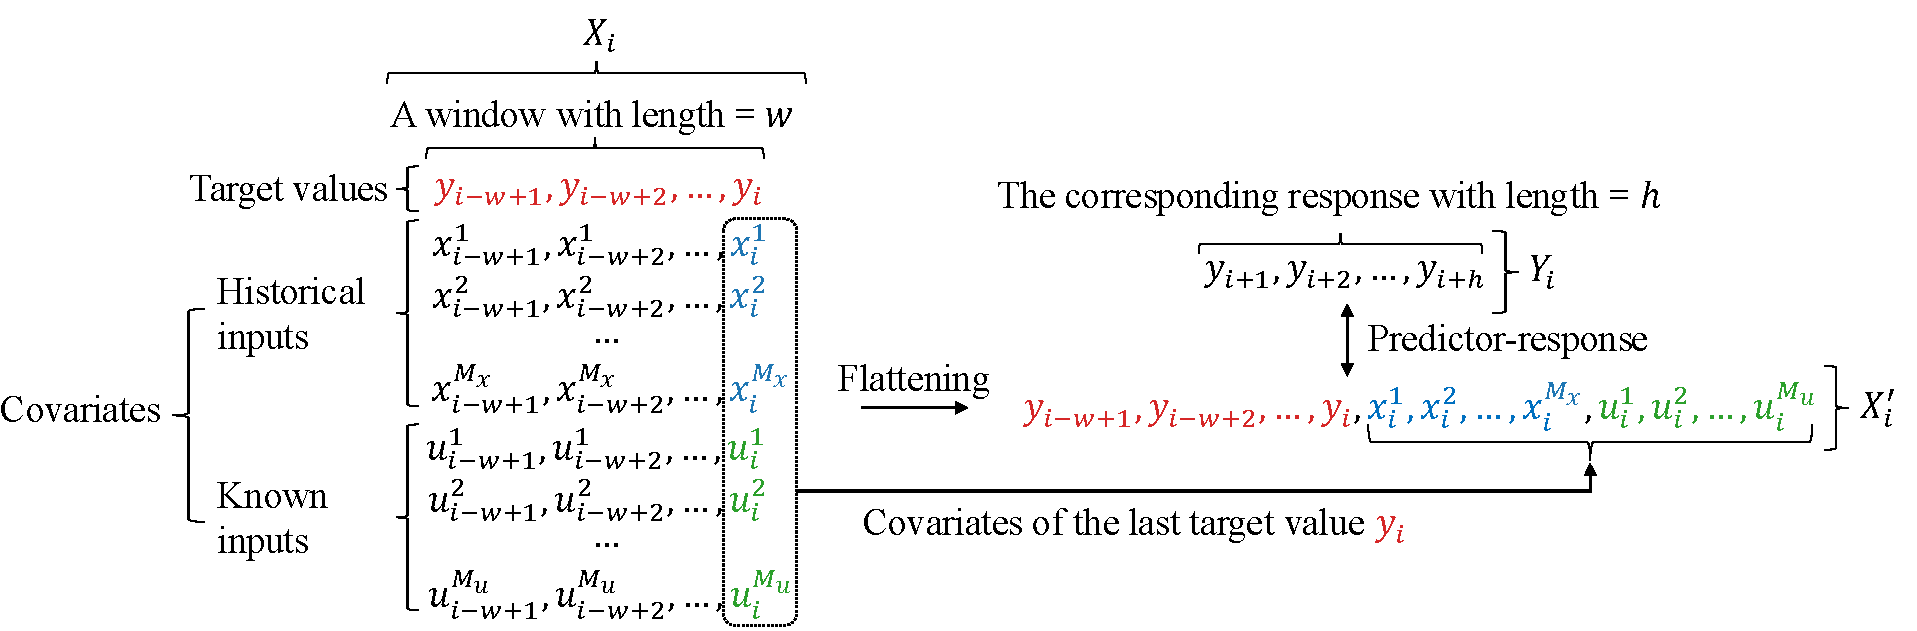
\includegraphics[width=1.0\columnwidth]{figures/flattening.pptx.pdf}}
\caption{
Flattening a 2D window $X_i$ of size $(1 + M_x + M_u) \times w$ to a 1D vector $X'_i$ of length $w + M_x + M_u$. 
The entries in the window are scalars.
$X'_i$ serves as the \textit{predictor} for the regressor. 
Its expected \textit{response} $Y_i$ is a vector of length $h$. 
The regressor learns from the predictor-response pairs.
}
\label{fig:flattening}
\end{figure*}